\ylDisplay{Pall} % Ülesande nimi
{Taivo Pungas} % Autor
{lõppvoor} % Voor
{2013} % Aasta
{G 2} % Ülesande nr.
{2} % Raskustase
{
% Teema: Dünaamika
\ifStatement
Madis analüüsis arvutiprogrammiga palli põrkamisest tehtud helilindistust
ja sai joonisel  toodud graafiku, mis näitab helisignaali kuju.
Kui on teada, et pärast kolmandat põrget tõusis pall täpselt \SI{1}{m} kõrgusele,
leidke palli maksimaalne kõrgus pärast esimest põrget.
\begin{center}
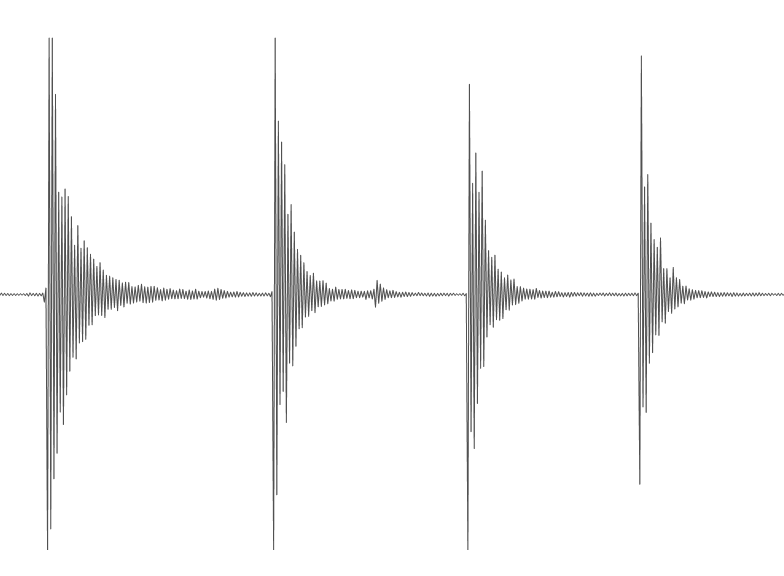
\includegraphics[width=0.5\textwidth]{2013-v3g-02-pall}%
\end{center}
\fi


\ifHint
Palli lennu kõrgus sõltub vastavale kõrgusele jõudmise aja ruudust.
\fi


\ifSolution
$h \propto t^{2}$, kus $h$ on maksimaalse tõusu kõrgus ja $t$ on sellele kõrgusele tõusmiseks kulunud aeg.\\
Olgu $t_{i}$ aeg, mis kulus pallil pärast $i$-ndat põrget maksimaalsele kõrgusele tõusmiseks. Kuna iga piik graafikul tähistab üht põrget, siis võime mõõta graafikult 3. ja 4. põrke alguste vahelise kauguse $d_{3}$, kusjuures $t_{3}=kd_{3}$ (kus $k$ on mingi võrdetegur), ning 1. ja 2. põrke alguste vahelise kauguse $d_{1}$, kusjuures $t_{1}=kd_{1}$. Seega 
$\frac{t_{1}}{t_{3}}=\frac{d_{1}}{d_{3}}$, kust
$$h_{1}=h_{3}(\frac{t_{1}}{t_{3}})^{2}=h_{3}(\frac{d_{1}}{d_{3}})^{2} \approx \SI{1,7}{m}.$$\\
\fi


\ifEngStatement
% Problem name: Ball
Madis studied an audio recording of a bouncing ball with a computer program and got a graph shown below which shows the shape of the audio signal. Find the maximal height of the ball after the first bounce if it is known that the ball rose exactly 1 m high after the third bounce.
\begin{center}
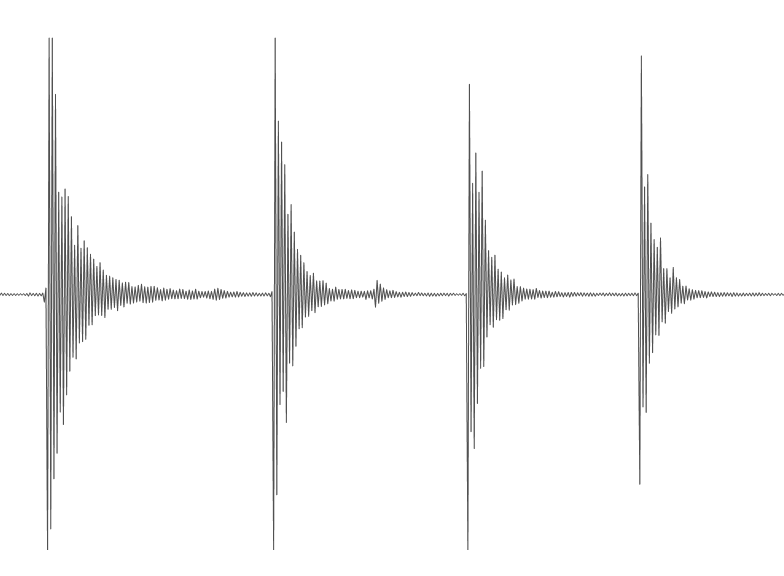
\includegraphics[width=0.5\textwidth]{2013-v3g-02-pall}%
\end{center}
\fi


\ifEngHint
The height of the ball’s flight depends on the squared time it takes to reach this height.
\fi


\ifEngSolution
$h \propto t^{2}$ where $h$ is the maximal height of the ball’s rise and $t$ is the time it took to reach that height.\\
Let $t_{i}$ be the time it took the ball to reach the maximal height after bouncing $i$ times. Because each peak in the graph marks one bounce then we can measure the distance $d_{3}$ between the beginnings of the third and fourth bounce, moreover $t_{3}=kd_{3}$ (where $k$ is some constant of proportionality) and the distance $d_{1}$ between the beginnings of the first and second bounce, moreover $t_{1}=kd_{1}$. Thus $\frac{t_{1}}{t_{3}}=\frac{d_{1}}{d_{3}}$ where 
$$h_{1}=h_{3}(\frac{t_{1}}{t_{3}})^{2}=h_{3}(\frac{d_{1}}{d_{3}})^{2} \approx \SI{1,7}{m}.$$
\fi
}